\chapter{Arquitectura}
\label{chap:arquitectura}

\noindent
\drop{E}{}n este capítulo se presentará la arquitectura del proyecto, planteando en primer lugar la estructura global, y analizando posteriormente las fases de desarrollo del proyecto, así como los componentes de este, y el proceso que se ha seguido para su diseño y desarrollo. También se explicará en detalle el sistema de recomendación que se ha implementado en este proyecto.

\section{Visión general}
En la Figura \ref{fig:arquitecture-diagram} se muestra una representación de estructura global del sistema. Por simplicidad y claridad, se muestra solo un módulo de la aplicación de usuarios, pese a que debería de haber dos para realizar la comunicación. Se puede comprobar en esta figura como los distintos módulos se comunican entre sí, y también las principales herramientas externas de las que hacen uso.


\begin{figure}[!h]
\begin{center}
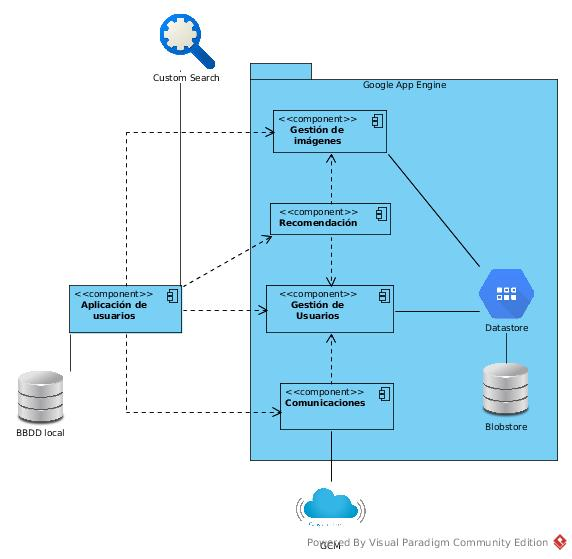
\includegraphics[width=1.1\textwidth]{./figures/arquitectura.jpg}
\caption[Arquitectura del sistema]{Arquitectura del sistema}
\label{fig:arquitecture-diagram}
\end{center}
\end{figure}


A continuación se analizarán los módulos del sistema:


\subsubsection{Módulo aplicación}
El principal propósito de la aplicación, es el de proporcionar una interfaz que presente las características necesarias para permitir al usuario comunicarse con otros, incluyendo el uso de imágenes. Esta interfaz será la encargada de interactuar con el usuario, presentándole todas las opciones de las que dispone el sistema. Gestionará tanto la configuración inicial del sistema como la posterior comunicación con otros usuarios. Se comunica con otros tres módulos. Utiliza el módulo de gestión de usuarios para gestionar el alta en el sistema del usuario y la sincronización con los contactos. El módulo de comunicaciones provee de los medios necesarios para enviar un mensaje a otro usuario. Finalmente el módulo de recomendación será empleado cuando el usuario quiera buscar una imagen, presentando una colección de posibles candidatas.


\subsubsection{Módulo de usuarios}
El módulo de usuarios es el encargado de gestionar toda la información relativa a los usuarios. Proporciona los mecanismos necesarios para poder dar de alta y sincronizar usuarios, así como para poder relacionar el número de teléfono de estos usuarios con el identificador necesario para poder hacer llegar el mensaje enviado por el usuario. Una vez obtenido el identificador envía el mensaje utilizando la \acs{API} \acs{GCM}. Otra labor importante de este módulo, es la de proporcionar la información relativa a los usuarios que sea necesaria para el modulo de recomendaciones, así como de actualizar esa información cuando existan cambios que así lo indiquen. 

\subsubsection{Módulo de comunicación}
Como su propio nombre indica, este módulo es el encargado de gestionar las comunicaciones entre los usuarios. Cuando el usuario envía un mensaje, este contendrá entre otras cosas el número de teléfono del destinatario así como toda la información relativa al mensaje. Este módulo se encargará de obtener el identificador necesario que debe proporcionar al sistema de \ac{GCM}, haciendo uso para ello del módulo de gestión de usuarios.


\subsubsection{Módulo de gestión de imágenes}
El principal propósito de este módulo es el de proporcionar una interfaz al módulo de recomendaciones, de manera que este tenga acceso las imágenes que se encuentran actualmente en el sistema, así como de proporcionar de una nueva fuente de imágenes. Permite filtrar estas imágenes según los criterios que establezca el sistema de recomendación, además de almacenar y actualizar la información necesaria para que el sistema de recomendación pueda aplicar los algoritmos correspondientes. También se encarga de almacenar en el Blobstore las nuevas imágenes.

\subsubsection{Módulo de recomendación}
Este es el módulo encargado de recomendar imágenes al usuario a partir de una entrada proporcionada por este. Analizando el perfil del usuario que proporcione el modulo de usuarios, así como la información relativa a las imágenes, este módulo filtrará entre aquellas imágenes que se encuentren actualmente disponibles en el sistema y las imágenes que proporcionen los mecanismos externos. También será el encargado de indicar al módulo de gestión de imágenes de los cambios que debe realizar sobre la información que contiene de estas. 















\section{Sistema de recomendación}
\label{sec:sistema-recomendacion}
El sistema de recomendación de imágenes es el componente más importante de este proyecto, y el que aporta a la aplicación de mensajería desarrollada la diferenciación respecto al resto que existen actualmente en el mercado. También es el componente que mayor complejidad computacional posee del proyecto, y por tanto se ha considerado necesario explicarlo con mayor detenimiento.


\subsection{Procesamiento de la entrada}
Atendiendo al carácter de la entrada es necesario aplicar un preprocesamiento de esta para poder tratar con ella. Esto es debido a que los usuarios pueden introducir la petición o consulta en un formato muy variado, ya que se trata de lenguaje natural.

\subsubsection{Limpieza de la entrada}


En primer lugar es necesario realizar una limpieza de la misma. En esta limpieza, entre otras cosas, se eliminarán aquellas palabras o elementos que no aporten nada, como las preposiciones, pronombres, artículos, etc., que se consideran \textit{palabras vacías} (stop words) dejando únicamente aquellas que aportan significado. 

Por otra parte, también se hace necesario tratar aquellas palabras que si han pasado el proceso de selección (nombres, verbos, adjetivos y adverbios), y preprocesarlas de manera que se eliminen las diferencias entre los plurales y los singulares (pasando todo a singular) o pasando los verbos a su forma en infinitivo.

Puede darse la situación en que al \textit{limpiar} aquellas palabras de elementos como prefijos o sufijos aparezcan varias opciones alternativas sobre las que esa palabra se puede reducir. En este caso se seguirá el criterio que establece Wordnet y se escogerá la primera opción por considerarse la más probable.

La salida de este proceso será la consulta que se utilice cuando se recurra a proveedores externos para buscar imágenes.\\


\subsubsection{Expansión de la entrada}


En segundo lugar encontramos el proceso de expansión de esta entrada. La primera razón por la que necesitamos ampliar esta entrada, es que diversos usuarios pueden hacer referencia al mismo elemento de diferentes maneras, por ejemplo, algunos pueden utilizar la palabra \textit{colegio} mientras que otros pueden utilizar \textit{escuela} refiriéndose a lo mismo, y la misma imagen puede ser perfecta para ambos usuarios. La segunda es debido al hecho de que se puede extraer información de estas palabras, que luego puede utilizarse a mediante conocimiento experto, para seleccionar distintos sitios web donde realizar la búsqueda. De esta manera, si tenemos conocimiento del tipo de contenido que aparece en un sitio web concreto, es muy útil que si el usuario introduce una consulta que sabemos que va a a aparecer en ese sitio, se realice una búsqueda ahí.

Por este motivo, se hace necesario procesar dicha entrada, buscando para todas aquellas palabras que han pasado el filtro inicial sinónimos e hiperónimos. Encontramos aquí un problema notable debido al hecho de que la mayoría de las palabras suelen tener varias acepciones, tanto en inglés como en español, y además una misma palabra puede ser a la vez un nombre, un verbo, un adjetivo y/o un adverbio. Esto implica que una misma palabra puede tener diferentes sinónimos o palabras relacionadas en función de aquella de las acepciones que tomemos.

Generalmente para nuestro caso no afectará aquella ambigüedad referente a la diferencia de verbo y nombre, ya que en inglés, aquellos nombres que se derivan de un verbo representan ese verbo, como por ejemplo \textit{run} en inglés, puede significar tanto correr como carrera, pero la imagen necesaria para representar el concepto representará normalmente tanto al nombre como al verbo. Respecto a esto, y debido a la naturaleza propia de las imágenes se escogerá siempre en primer lugar la acepción referente a los nombres, ya que será aquella con la que más se trabaje. En caso de no existir una definición referente a esa palabra como nombre, lo cual implicaría que esa palabra nunca puede ser un nombre, se recurriría en segundo lugar a las acepciones de verbo, en caso de que tampoco existan acepciones de esa palabra que sean verbos se recurriría a adjetivos y finalmente si esto tampoco funciona a adverbios. 

Respecto a la existencia de varias acepciones de la misma forma gramatical, es donde surgen mayores problemas. Volviendo al caso de antes, \textit{run} en inglés, puede significar una simple carrera realizada a pie, o, en el contexto del fútbol americano, una jugada en la que un jugador intenta pasar el balón a través del equipo contrario, además de otras muchas acepciones como sustantivo. En numerosas ocasiones, esta diferencia de definición hace referencia a palabras que han adquirido el mismo nombre por ciertas relaciones semánticas o históricas, y aunque distintas es su definición exacta, están muy relacionadas, por lo que la selección de una acepción no es tan crucial. Sin embargo, en muchos otros casos, las diferentes acepciones no se limitan a este tipo de relaciones, y una misma palabra puede referirse a dos conceptos muy distintos. Por ejemplo, la palabra \textit{mean} como adjetivo puede significar tanto ser mezquino, como la media estadística. 

En el caso de este proyecto y atendiendo a sus limitaciones, se ha decidido recurrir a la opción de escoger la primera acepción que aparezca en cada caso. Como se verá más adelante, aquí es donde nos encontramos con una de las posibilidades más interesantes de mejora del sistema, tanto para reconocer la forma gramatical de la que se trata, como para reconocer a partir del contexto su significado semántico, pudiendo aplicar para ello procedimientos más sofisticados. 

Respecto a la aplicación de los sinónimos, se utilizarán únicamente con aquellos recursos que se encuentren en el sistema. Esto quiere decir que no se utilizarán estas palabras extras en las búsquedas de proveedores externos. El motivo de este mecanismo de actuación, es debido a que sería computacionalmente muy costoso (con todo lo que ello conlleva) aplicar estos mecanismos a la búsqueda por ejemplo en \acs{GSE}, ya que para cada palabra sería necesario realizar una nueva búsqueda, con todo lo que ello conlleva. Además, en este caso, Google ya realiza un procesamiento propio en las búsquedas. Si bien, cuando un usuario seleccione una imagen que proceda de un medio ajeno, y esta se incluya en el sistema, en este caso si se incluirán estas nuevas palabras como palabras clave de la imagen. A continuación, se mostrarán los diferentes perfiles relevantes para el sistema de recomendación, así como las técnicas aplicadas, y se podrá observar con más detalle como se tratan todas estas nuevas palabras a las que se llamará palabras clave.

Los hipónimos por su parte, se utilizarán para seleccionar aquellos sitios web, que previo análisis hayan sido etiquetados con uno de estos hiperónimos o categorías.

\subsection{Técnicas empleadas}
En esta sección se presentarán las técnicas empleadas que se vieron en la Sección \ref{sec:tecnicas-recomendacion}, así como los mecanismos de hibridación utilizados para combinar estas técnicas.

En primer lugar es necesario indicar que el contenido de las valoraciones en este caso será principalmente binario, considerándose la selección de una imagen como valoración positiva y la no selección como negativa. Sin embargo, en este proyecto se usará únicamente la información referente a las valoraciones positivas, es decir, se tendrá en cuenta para los diferentes algoritmos únicamente la información correspondiente a las imágenes utilizadas por los usuarios.

Respecto a las técnicas de recomendación empleadas son las siguientes:\\

\subsubsection{Basada en contenido}


Por un lado tenemos la técnica de recomendación basada en contenido. Como se ha mencionado anteriormente, esta tipo de técnica busca relaciones entre elementos que ya han sido positivamente valorados por el usuario y los nuevos elementos que están en el proceso de selección para la recomendación, y escoge aquellos que según cierto criterio más se asemejen a los ya valorados.

En este caso, esta técnica valorará la información sobre las imágenes que ya han sido seleccionadas por el usuario, comprobando si existe relación entre estas, y creando un perfil para este usuario. Así, el perfil de una imagen usada (\textit{ImagenUsada}) por un usuario estará compuesto del identificador de la imagen, junto con un contador del número de veces que ha utilizado esa imagen. 

Por otra parte la información relativa a la \textit{Imagen}, la cual podemos identificar como el perfil de la imagen, será la que se muestra a continuación:

\begin{itemize}
\item identificador\textunderscore blob: Es el identificador que permite recuperar la imagen que esta almacenada en el Blobstore.
\item etiquetas: Las etiquetas que proporciona Google Cloud Vision sobre la imagen.
\item palabras\textunderscore clave: Las palabras utilizadas en las búsquedas por los usuarios que hayan seleccionado esa imagen. Esto incluye también aquellas palabras relacionadas que se han extraído utilizando la herramienta Wordnet.
\item enlace: El enlace completo donde se encontraba el recurso originalmente.
\item enlace\textunderscore sitio: El enlace del sitio web de cual se tomó la imagen.
\end{itemize}

Se usará la información referente a los sitios web para conocer las preferencias y gustos de los usuarios por ciertos sitios web en concreto. Esto se usará en las búsquedas de nuevas imágenes, especificando búsquedas en aquellos sitios web que contienen o contenían imágenes previamente seleccionadas por este. Estos perfiles o entidades ayudarán a comprender la estructura del sistema, así como a entender el funcionamiento del algoritmo que se describirá más adelante.\\

\subsubsection{Colaborativa}


También se va a aplicar la técnica colaborativa. Esta técnica establece relaciones entre los usuarios basándose en los elementos que han valorado previamente. Posteriormente, cuando un usuario solicita una recomendación o el sistema le ofrece una, se analiza la relación existente entre ese usuario y otros que hayan valorado ítems en los que el usuario pueda estar interesado, y le recomienda uno o varios de estos ítems.

Respecto a la adaptación de esta técnica en este proyecto, la relación entre los usuarios se medirá atendiendo a las imágenes que estos han utilizado (en este caso es lo mismo que valorar positivamente). 

Se valorará una única vez el hecho de que dos usuarios utilicen una misma imagen, es decir, si ambos usuarios valoran positivamente la misma imagen varias veces, a efectos de la relación existente entre estos usuarios para esta técnica, será igual que si ambos han valorando positivamente la imagen una única vez. Esto se hace de esta manera para que una sola imagen introduzca tanto ruido que ambos usuarios parezcan similares al sistema pese a que solo coincidan en esto. Así pues, el grado de relación o de semejanza entre dos usuarios se medirá en función del número de imágenes en común que estos hayan utilizado.

Para cada relación de usuarios (\textit{UsuariosRelacionados}) se creará una entidad que contenga un identificador de cada usuario junto con el grado de relación existente entre ellos. El perfil de un \textit{Usuario} está determinado por lo siguiente:

\begin{itemize}
\item numero\textunderscore telefono: Número de teléfono del usuario.
\item identificador\textunderscore comunicaciones: Identificador de registro, necesario para el sistema de comunicaciones
\item palabras\textunderscore clave: Utilizadas por los usuarios en sus búsquedas. Esto incluye también aquellas palabras relacionadas que se han extraído utilizando la herramienta Wordnet.
\item imagenes\textunderscore utilizadas: identificador de la imagen junto con un contador).
\end{itemize}

Además de estas relaciones, existen otras que son auxiliares a estas y que utilizarán en el pseudocódigo. Están las \textit{PalabrasClave}, que contienen una palabra clave junto con el número de veces que ha sido empleado. Y por último la \textit{Etiqueta}, que contiene una etiqueta proporcionada por Google Cloud Vision junto con una probabilidad que este aporta de que el término se corresponda con la imagen. 

En el Listado \ref{code:imagenSeleccionadaPseudo} se muestra el pseudocódigo referente a los procesos que se ejecutan cada vez que una imagen es seleccionada, y que modifican la información referente a esa imagen y al usuario, así como a las relaciones entre estos. Este pseudocódigo, al igual que los demás mostrados en esta sección, muestran una versión simplificada, aislando de los detalles de la implementación y la tecnología usada, y mostrando únicamente el proceso de manera más abstracta.

Cada vez que se seleccione una imagen, se comprueba si esta ya se encuentra en el sistema. En caso de no encontrarse aún, crea un blob para almacenarla, y la sube al sistema. Además añade la información que será estática en el sistema, como son el enlace, enlace del sitio y las etiquetas de Google Cloud Vision, que aportarán información similar a la proporcionada por las palabras clave que hayan utilizado los usuarios. Después, y al igual que haría si la imagen existiese en el repositorio propio, actualiza la información referente a las palabras clave que han sido empleadas como se muestra en el Listado \ref{code:actualiza-palabras-clave}. Esta actualización se hace tanto para la imagen como para el propio usuario, ya que cada perfil lleva un registro de las palabras utilizas (por uno en el caso del usuario y empleadas en el otro en el caso de la imagen), junto con el número de veces que se han empleado. En el pseudocódigo mostrado, solo existe un método de actualización que será válido para los dos tipos de entidades. De esta manera, si no se han utilizado nunca se añaden con valor uno, y si ya han sido utilizadas se incrementa el contador.\\

\lstinputlisting[texcl, caption = {Actualización de la información tras la selección de una imagen}, language = Python, label = code:imagenSeleccionadaPseudo]{code/imagenSeleccionadaPseudo.py}

\lstinputlisting[texcl, caption = {Actualización de las palabras clave de usuarios e imágenes}, language = Python, label = code:actualiza-palabras-clave]{code/actualiza-palabras-clave-pseudo.py}


Además de actualizar las etiquetas es necesario realizar otras modificaciones respecto de las relaciones existentes entre los usuarios (Listado \ref{code:actualiza-usuarios-relacionados}), y entre los usuarios y las imágenes que han utilizado (Listado \ref{code:actualiza-imagenes-utilizadas}). Cada usuario tiene un registro de las imágenes que este ha seleccionado junto con el número de veces que lo ha hecho, y por tanto se actualiza cada vez que se añade una imagen en caso de que ya la haya utilizado alguna vez, o por el contrario se crea una nueva referencia inicializando el contador.

Respecto a la relación entre usuarios, como se ha mencionado anteriormente, por cada imagen que dos usuarios tienen en común, su relación gana fuerza.\\ 

\lstinputlisting[texcl, caption = {Actualización de las imágenes utilizadas por un usuario}, language = Python, label = code:actualiza-imagenes-utilizadas]{code/actualiza-imagenes-utilizadas-pseudo.py}

\lstinputlisting[texcl, caption = {Actualización de la relación entre usuarios}, language = Python, label = code:actualiza-usuarios-relacionados]{code/actualiza-usuarios-relacionados-pseudo.py}

\subsubsection{Basada en conocimiento}

Este tipo de técnicas realiza una recomendación a partir del conocimiento de como un determinado elemento cumple con los requisitos del usuario. En este caso, ese conocimiento es el tipo de imágenes que se pueden encontrar principalmente en según que sitios web. De esta manera, puede ser que uno de los sitios donde se realiza la búsqueda este principalmente orientado a imágenes de animales, mientras que otro lo este a imágenes de actividades deportivas. Debido a que se utilizarán imágenes que se encuentran en sitios web externos al sistema, es posible adquirir conocimiento sobre esos sitios y descubrir si esos sitios poseen imágenes que se especializan en algún campo en concreto. De este modo, cuando un usuario realice una búsqueda que este relacionado con alguno de estos temas, será posible proporcionarle la opción de buscar específicamente en sitios donde seguro que hay imágenes que le serán de utilidad.

Esto, es posible mediante la expansión de la entrada realizada anteriormente, obteniendo una serie de hiperónimos que podremos asociar con las categorías a las que hemos asociado algunas páginas web.  Los hiperónimos de una palabra representan aquellas que de alguna manera, representan un concepto que engloba a esta palabra. De esta manera, por ejemplo en el caso de la palabra perro o \textit{dog} en inglés, tenemos que uno de sus hiperónimos es \textit{canine}, que hace referencia a aquellos animales que descienden de los lobos. Esto en principio no aporta demasiada utilidad debido a que no será común encontrarnos páginas de lobos y perros exclusivamente. Pero además de este, otro de los hiperónimos que encontramos es \textit{domestic\textunderscore animal}. Este, a diferencia del anterior si resulta muy útil, ya que podemos disponer de sitios web que contengan fotos de animales domésticos como perros y gatos.

Se recogerán en un archivo de configuración que podrá ser modificado fácilmente, algunos de los sitios web disponibles para las búsquedas, junto con las categorías que destacan en cada uno de los sitios.


%Si aplicamos lo de hiepronimos o algo de eso se puede hacer basada en conocimiento
\subsubsection{Hibridación}


Por último, se hace necesario aplicar alguno de los mecanismos de hibridación vistos en la Sección \ref{sec:sistemas-hibridos} para combinar las técnicas que se han decidido utilizar. En este caso se ha decidido emplear un sistema conmutado. En este tipo de sistemas, se combinan en la salida recomendaciones de todas las técnicas que se emplean, pudiendo aportar cada una de las técnicas un mayor o un menor número de elementos en función del mecanismo que se decida implantar.

En este caso, se ha decidido utilizar este mecanismo debido a que las recomendaciones proporcionadas por todas las técnicas son útiles en todo momento, ya sea en mayor o menor medida. Siempre será útil disponer de nuevas imágenes de manera que el sistema no sufra de sobreespecialización y se quede estancado con las imágenes que tenga, y será necesario buscar estas para lo que la técnica basada en contenido será de gran utilidad. Posteriormente, cuando la cantidad de imágenes de las que se disponga en el repositorio propio empiece a aumentar también irá siendo cada vez más útil aquellas imágenes proporcionadas por la técnica colaborativa. De esta manera, permite adaptar en cada momento que técnica tiene mayor relevancia, y dar mayor peso a esta, sin dejar de aprovechar las ventajas que aportan las demás. 

Cuando el sistema comienza a funcionar únicamente se dispone de las primeras imágenes que se encuentran en el sistema que son los pictogramas, de aquellas proporcionadas por los proveedores externos y de la información proporcionada por la técnica basada en conocimiento. De esta manera, al comienzo de su puesta en marcha, el sistema será poco más que un sistema de filtrado de imágenes, sin aportar ningún rasgo de personalización a los usuarios.

Conforme el usuario empiece a utilizar en mayor medida el sistema, este será capaz de aprender de los gustos de los usuarios y comenzarán a cobrar mayor importancia, lo cual resultará en mayor número de imágenes aportadas por este tipo de técnica en la salida final que se le proporcionará al usuario. Al igual que en este caso, cuando el número de usuarios se expanda, y aumente la relación entre estos, será la técnica colaborativa la que pase a aportar mayor peso en las recomendaciones.


\subsection{Algoritmo}

Respecto al algoritmo de recomendación, se mostrarán una serie de listados mostrando un pseudocódigo de cada una de las técnicas aplicadas y como se han aplicado. En el Listado \ref{code:algoritmo-recomendacion} se muestra lo que sería el proceso de combinación de los resultados proporcionados por las diferentes técnicas. 

En primer lugar, aparecen los valores de unas constantes que nos permitirán configurar el número máximo de imágenes que se recomendarán al usuario en total, así como el máximo número de imágenes que proporcionará cada uno de las técnicas de recomendación. Más adelante, se verá como existen mecanismos para controlar que si una técnica no es lo suficientemente confiable con los datos que tiene, aportará menos imágenes de este máximo. Los valores de estas constantes se pueden adaptar en caso de considerarse necesario dar más importancia a alguna de estas técnicas.

En el caso de la técnica colaborativa por ejemplo, es necesario establecer un valor mínimo para la relación entre los usuarios, ya que si no, puede darse el caso de que ambos hayan valorado tan solo unas pocas imágenes en común por casualidad pero sus gustos difieran enormemente. Lo mismo ocurre con la técnica basada en contenido, sí el usuario ha seleccionado imágenes de numerosos portales y no tiene una clara predilección por ninguno, esta técnica puede no aportar valor útil.\\

\lstinputlisting[texcl, caption = {Algoritmo de recomendación}, language = Python, label = code:algoritmo-recomendacion]{code/algoritmo-recomendacion.py}

Usando la aplicación de la técnica colaborativa (Listado \ref{code:algoritmo-colaborativo} se procederá en primer lugar a obtener aquellas imágenes que contienen las palabras clave que el usuario ha introducido. Posteriormente se obtendrán todos aquellos usuarios que hayan seleccionado en algún momento alguna de las  imágenes que se encuentran el la selección anterior, es decir, que hayan seleccionado imágenes que contenga alguna de las palabras clave que se encuentren en la búsqueda. A continuación, se obtendrá el conjunto de los usuarios que estando relacionados (mediante el procedimiento explicado anteriormente), también se encuentren en el conjunto de usuarios que hayan valorado imágenes que contengan las palabras clave de la consulta. Este conjunto que contiene los usuarios relacionados, estará ordenado por la fortaleza entre la unión de ambos.

Así, para cada usuario de este conjunto, y hasta que no se alcance el número de imágenes mínimo, o la relación de usuarios deje de ser lo suficientemente relevante como para considerar que ambos usuarios no están lo suficientemente relacionados, se seleccionará de cada usuario aquella imagen que conteniendo alguna de las palabras clave, haya sido empleada mayor número de veces por el usuario en cuestión. Además el sistema se asegurará de que no se introducen imágenes repetidas en el conjunto de salida.\\

\lstinputlisting[texcl, caption = {Algoritmo de la técnica colaborativa}, language = Python, label = code:algoritmo-colaborativo]{code/algoritmo-colaborativo.py}


El algoritmo que aplica la técnica basada en contenido (Listado \ref{code:algoritmo-contenido}, en primer lugar obtendrá las imágenes utilizadas por el usuario. Para cada una de estas imágenes comprobará el sitio web en el que se encontraban, elaborando una lista con todos los sitios así como del número de veces que el usuario ha seleccionado una imagen de ese sitio. Tras ordenar esta lista, seleccionará los sitios que han sido más recurridos por el usuario y dentro de los límites que se hayan delimitado para esta técnica, y comprobará si es lo suficientemente relevante, para lo cual comprobará si el número de imágenes que se han extraído de ese portal es superior al doble de la mediana de las veces que ha visitado cada portal.\\

\lstinputlisting[texcl, caption = {Algoritmo de la técnica basada en contenido}, language = Python, label = code:algoritmo-contenido]{code/algoritmo-contenido.py}

Finalmente, se aplicará la técnica basada en conocimiento (Listado \ref{code:algoritmo-conocimiento}, la cual comprobará si alguna de las categorías en las que se agrupan los elementos de la entrada, se encuentran recogidas en el archivo de configuración que recoge sitios web junto con las categorías específicas de su contenido. En caso de que alguna de estas categorías se encuentre en este conjunto, se devolverá el sitio web que tiene asociado.\\

\lstinputlisting[texcl, caption = {Algoritmo de la técnica basada en conocimiento}, language = Python, label = code:algoritmo-conocimiento]{code/algoritmo-conocimiento.py}

La salida, como se puede comprobar en el Listado \ref{code:recommend-json}, será un archivo json que será enviado al usuario, para que este pueda tanto realizar la búsqueda de las imágenes en esos portales, como la búsqueda de las imágenes genérica para completar el total de imágenes necesarias para recomendar. Esta búsqueda será realizada y gestionada directamente por el dispositivo del usuario, de manera que se libere de carga al servidor, y disminuya a la vez la carga en la red, lo cual permitirá ahorrar tanto recursos como por consiguiente dinero en caso de que por motivos de la demanda de usuarios y uso sea necesario pasar a hacer uso de algunas versiones de pago de las tecnologías usadas. El orden en el que se le presentarán las imágenes al usuario será tal cual se descarguen en el dispositivo y muestren, es decir, no existirá un orden específico.\\

\lstinputlisting[texcl, caption = {JSON de salida del sistema de recomendación}, language = json, label = code:recommend-json]{code/recommendResult.json}


























\section{Fases de desarrollo}

A lo largo de esta sección, se mostrarán las diferentes iteraciones o sprints que se han llevado a cabo para desarrollar este proyecto. Estos sprints se derivan de la planificación inicial establecida en el Capítulo \ref{chap:metodo}, en concreto se puede observar dicha planificación en el Cuadro \ref{tab:user-stories}. Para cada sprint se mostrarán las Historias de Usuario que se han seleccionado (Sprint Backlog), mostrando estas en detalle, y desglosándolas en tareas. Se analizarán estas tareas mostrando cuando sea preciso el código desarrollado para implementar esta tarea, así como los diagramas que se considere oportuno para aclarar las diferentes tareas.

\subsection{Sprint 1}

En el sprint planning meeting se ha decidido que para este sprint se realizarán la primera y segunda \ac{HU}. En los Cuadros \ref{tab:user-story-1} y \ref{tab:user-story-2} se muestra el Sprint Backlog, con las Historias de Usuario seleccionadas para esta interacción, indicando entre otras cosas los mecanismos de validación, así como las tareas en las que se desglosa, y el tiempo estimado para su realización.

\begin{table}[hp]
  \centering
  {\small
  \begin{tabular}{|p{0.4\textwidth} |p{0.4\textwidth} |}
\hline
\multicolumn{2}{|l|}{\cellcolor[HTML]{C0C0C0}{\textbf{Historia de usuario}}} \\ \hline
\textbf{Número:} 1           & \textbf{Rol:} Usuario           \\ \hline
\textbf{Esfuerzo:}          & \textbf{Iteración:} 1         \\ \hline
\multicolumn{2}{|p{0.8\textwidth}|}{\textbf{Nombre:} Aplicación Android } \\ \hline
\multicolumn{2}{|p{0.8\textwidth}|}{\textbf{Desarrollador responsable:} Victor Gualdras de la Cruz} \\ \hline
\multicolumn{2}{|p{0.8\textwidth}|}{\textbf{Descripción:}\newline
Como usuario quiero poder acceder a una aplicación Android que presente las características y funcionalidades básicas de una aplicación de mensajería} \\ \hline
\multicolumn{2}{|p{0.8\textwidth}|}{\textbf{Validación:}\newline
Los usuarios pueden instalar la aplicación en su dispositivo y navegar por la aplicación, realizando acciones como escribir a contactos que serán falsos y se insertarán de manera manual.} \\ \hline
\multicolumn{2}{|p{0.8\textwidth}|}{\textbf{Tareas:}\newline
Tarea: Interfaz de instalación.\newline
Tarea: Interfaz genérica de la aplicación.\newline
Tarea: Diseñar e implementar base de datos local.\newline
Tarea: Simular usuarios para poder probar la interfaz.
}\\ \hline
\end{tabular}
  }
  \caption{Historia de Usuario 1}
  \label{tab:user-story-1}
\end{table}

\begin{table}[hp]
  \centering
  {\small
  \begin{tabular}{|p{0.4\textwidth} |p{0.4\textwidth} |}
\hline
\multicolumn{2}{|l|}{\cellcolor[HTML]{C0C0C0}{\textbf{Historia de usuario}}} \\ \hline
\textbf{Número:} 2        & \textbf{Rol:} Usuario          \\ \hline
\textbf{Esfuerzo:}           & \textbf{Iteración}: 1       \\ \hline
\multicolumn{2}{|p{0.8\textwidth}|}{\textbf{Nombre:} Entrada por texto y por voz} \\ \hline
\multicolumn{2}{|p{0.8\textwidth}|}{\textbf{Desarrollador responsable:} Victor Gualdras de la Cruz} \\ \hline
\multicolumn{2}{|p{0.8\textwidth}|}{\textbf{Descripción:}\newline
Como usuario quiero poder realizar la entrada metiante texto y voz en una conversación, así como que mis mensajes se guarden al enviar.} \\ \hline
\multicolumn{2}{|p{0.8\textwidth}|}{\textbf{Validación:}\newline
El usuario podrá seleccionar un contacto con el que simular una conversación. Podrá seleccionar la vía escrita o mediante voz, y al pulsar en enviar verá como el mensaje aparece en la pantalla. Si sale y vuelve a entrar el mensaje seguirá ahí.} \\ \hline
\multicolumn{2}{|p{0.8\textwidth}|}{\textbf{Tareas:}\newline
Tarea: Realizar la entrada mediante texto y mediante voz.\newline
Tarea: Almacenar mensajes y visualizarlos como si se hubiesen enviado.
} \\ \hline
\end{tabular}
  }
  \caption{Historia de Usuario 2}
  \label{tab:user-story-2}
\end{table}

\subsubsection{Tarea: Interfaz de instalación}

Será necesario desarrollar una interfaz que se ejecutará tras la instalación de la aplicación en el dispositivo. Consistirá en una ventana en la que aparecerá un cuadro de texto donde escribir el número de teléfono, junto con un desplegable donde aparecen los prefijos internacionales. La aplicación detectará automáticamente la nacionalidad de la tarjeta SIM, fijando directamente el prefijo. Aún así, el usuario podrá seleccionar otro si así lo considera.

Esta pantalla inicial permitirá en un futuro realizar acciones antes de comenzar a ejecutar la aplicación, como registrar al usuario en algún servicio si así fuese necesario. En la Figura \ref{fig:interfaz-instalacion} la primera imagen muesra esta interfaz.


\subsubsection{Tarea: Interfaz genérica de la aplicación}

Esta será la interfaz que el usuario utilizará tras la configuración inicial. Se ha diseñado una interfaz orientada a la adición de una mayor funcionalidad en el futuro que la convierta de manera progresiva en una aplicación de mensajería mas completa y más usable. La vista principal consistirá de una lista donde el usuario podrá ver a aquellos que el tiene como contactos. En caso de que el usuario tenga asignada una imagen para ese contacto en el teléfono esta será la utilizada por la aplicación. En caso de no tener ninguna imagen asignada se utilizará una por defecto. El nombre del contacto también sera aquel que aparezca en la información del contacto almacenada por el usuario. En la Figura \ref{fig:interfaz-instalacion} se muestra en la segunda imagen la composición de la interfaz principal.

Todas aquellas cadenas de texto que aparezcan a lo largo de la interfaz estarán configuradas para que se adapten al idioma por defecto del teléfono. Aunque como ya se comentó al principio, la aplicación está orientada al inglés, se realiza de esta forma en caso de que en un futuro se decida ampliar el alcance de la misma.

\begin{figure}[!h]
\begin{center}
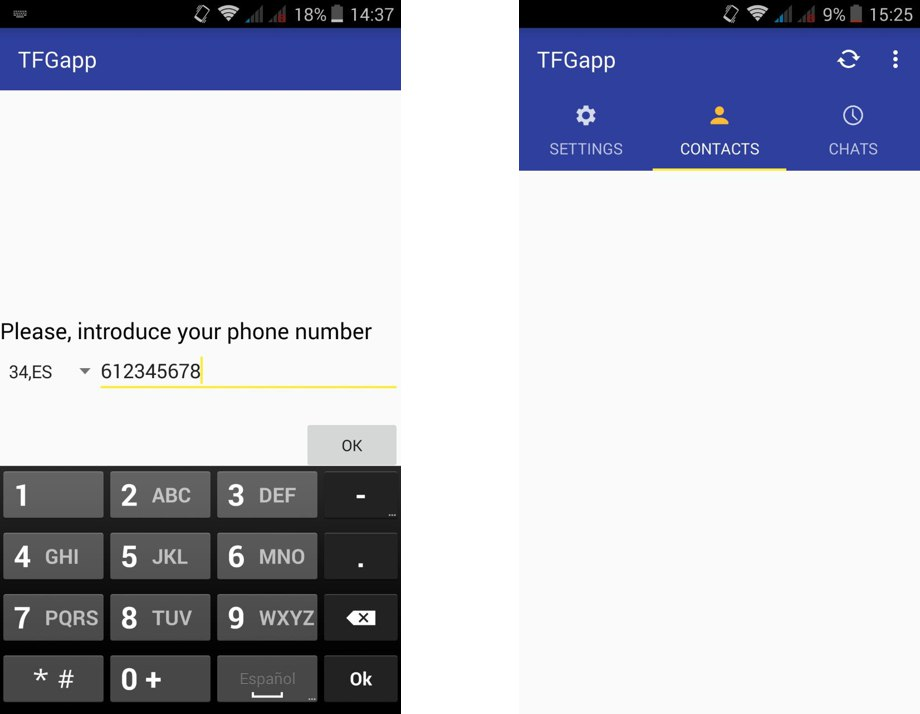
\includegraphics[width=0.9\textwidth]{./figures/interfaz-instalacion.jpg}
\caption[Interfaz de instalación y genérica]{Interfaz de instalación y genérica}
\label{fig:interfaz-instalacion}
\end{center}
\end{figure}


\subsubsection{Tarea: Diseñar e implementar base de datos local}

Será necesario la utilización de una base de datos local que nos permita almacenar la información relativa a los contactos que el usuario tiene. Se utilizará la clase SQLiteDatabase proporcionada por Android para almacenar los datos. Para el acceso a la base de datos se usará la clase ContentProvider, la cual proveerá de una interfaz para acceder a estos datos, y realizar las operaciones pertinentes. El código referente a la \ac{BBDD} se encuentra en la clase \textit{DavaProvider.java}, en el paquete de persistencia del código referente a la aplicación. A continuación se muestran los campos que componen la tabla referente a los perfiles contactos, la cual se llama profile.
\begin{itemize}
\item \textbf{\textunderscore id:} será un entero generado automáticamente de manera incremental, y que será la clave primaria.
\item \textbf{Name:} Un campo de tipo texto que contendrá el nombre de cada usuario y que será el que se muestre.
\item \textbf{phoneNumber:} Campo de tipo texto y único. Contendrá el teléfono del usuario.
\item \textbf{photo:} Campo de tipo texto. Contendrá la ruta relativa al lugar donde se encuentra almacenado el archivo deseado.
\end{itemize}

Además, la clase ContentProvider proveerá de una funcionalidad muy importante, y es la de que permitirá que cada vez que se modifique la base de datos, automáticamente se actualice la interfaz que presenta los datos relativos a los contactos. 


Para este refresco de la interfaz también será necesario hacer uso de clase CursorLoader, que será el encargado de realizar las consultas en segundo plano (evitando bloquear la interfaz) sobre el ContentProvider, y que estará integrado con la interfaz. Este CursorLoader establecerá aquella información que será necesario consultar y retornar.Esta clase a su vez devolverá un cursor, que a su vez proporcionará a las vistas con la información necesaria para actualizarse. En el Listado \ref{code:ContactTab} se puede observar como funciona este proceso. Debido a la gran cantidad de código que contenía la clase referente a este listado, se ha eliminado aquello que no se ha considerado relevante, pero como se ha mencionado en la introducción puede consultarse en el CD. \\


\lstinputlisting[texcl, caption = {Refresco de la interfaz tras modificación \acs{BBDD}}, language = Java, label = code:ContactTab, firstline=38]{code/ContactTab.java}

\subsubsection{Tarea: Simular usuarios para poder probar la interfaz}

Se añadirá la información de los usuarios simulada en la base de datos para comprobar que todo funciona correctamente. Servirá tanto para comprobar que los usuarios se muestran correctamente como para comprobar que las conversaciones también se comportan conforme a lo establecido. En la Figura \ref{fig:interfaz-contactos} se muestra el resultado.


\begin{figure}[!h]
\begin{center}
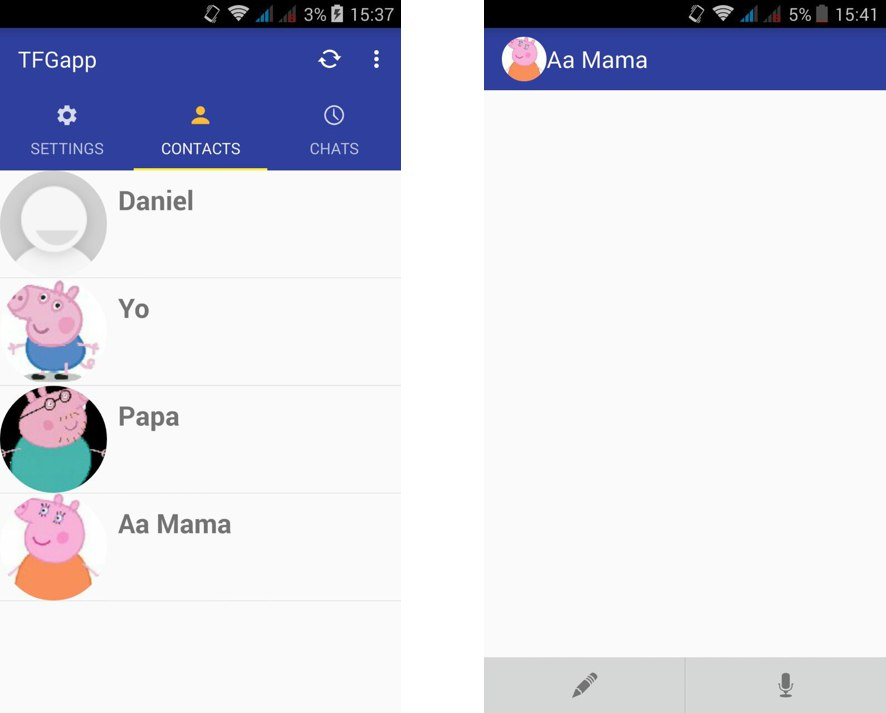
\includegraphics[width=0.9\textwidth]{./figures/interfaz-contactos.jpg}
\caption{Interfaz de contactos y conversaciones}
\label{fig:interfaz-contactos}
\end{center}
\end{figure}

\subsubsection{Tarea: Realizar la entrada mediante texto y mediante voz}

En la conversación entre usuarios, estos podrán seleccionar tanto entrada mediante texto como por voz, y podrán intercambiar los métodos durante las mismas en el momento que deseen. La entrada por voz se realizará mediante 


\subsubsection{Tarea: Almacenar mensajes y visualizarlos}

Será necesario crear una nueva tabla en la base de datos para los mensajes junto con la tabla de los usuarios. Se seguirá el mismo mecanismo que en el caso de los contactos, actualizando la interfaz de mensajes de manera muy similar a la empleada con los contactos por lo que no se volverá a mostrar el código. La información sobre los campos de esta tabla es la siguiente:

\begin{itemize}
\item \textbf{\textunderscore id:} será un entero generado automáticamente de manera incremental, y que será la clave primaria.
\item \textbf{msg:} Campo de tipo texto con el contenido del mensaje. En caso de tratarse de un archivo multimedia contendrá la ruta en la que se encuentra dicho archivo.
\item \textbf{type:} Tipo texto que indica el tipo del mensaje, texto o imagen en este caso.
\item \textbf{phoneNumberFrom:} Texto que contiene el número de teléfono que ha enviado el mensaje en caso de ser un mensaje recibido o el propio en caso de ser enviado.
\item  \textbf{phoneNumberTo:} Es un campo en formato de texto con el número de teléfono del destinatario del mensaje en caso de ser un mensaje enviado o nulo en caso de ser recibido.
\item \textbf{at:} Campo en formato datatime que contiene el momento en el que se recibió o envió el mensaje. Se establece de manera automática al almacenar un mensaje en la \ac{BBDD}.
\end{itemize}

En la Figura \ref{fig:interfaz-conversacion} se puede comprobar en que consisten los dos tipos de entrada y como se muestran los mensajes.


\begin{figure}[!h]
\begin{center}
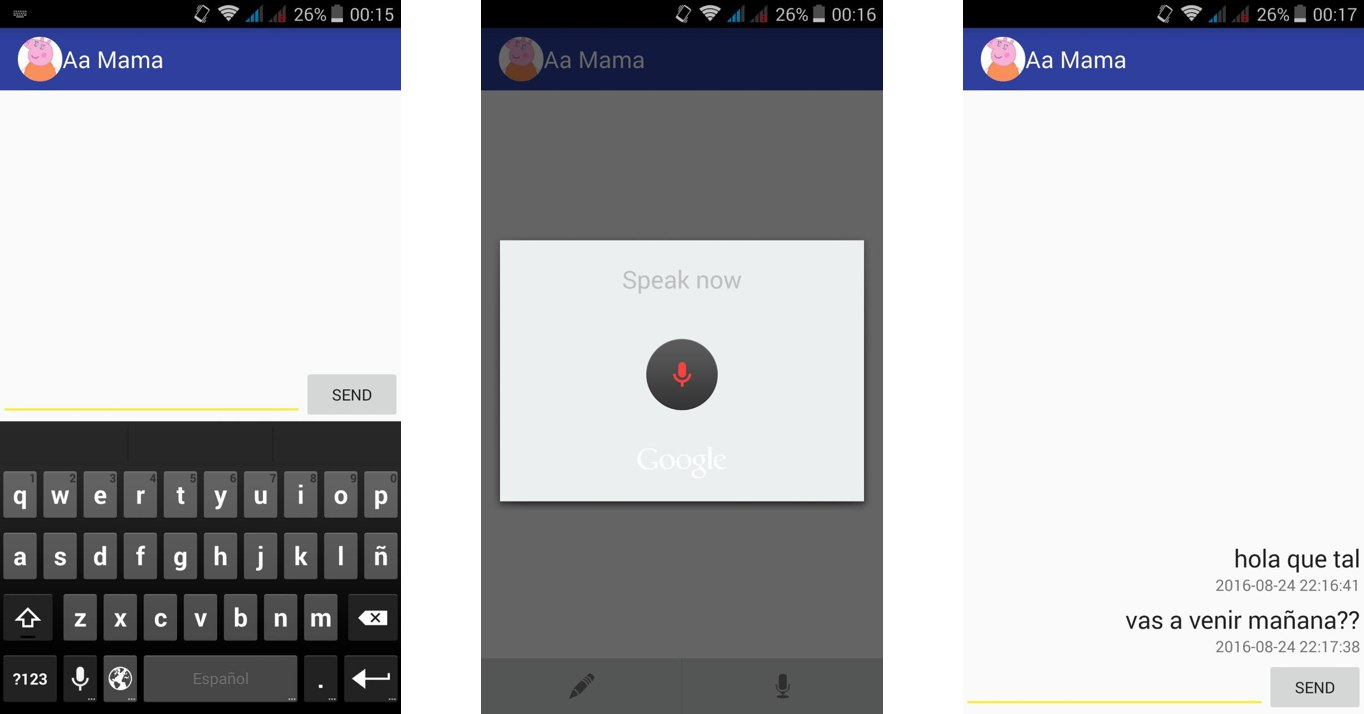
\includegraphics[width=1\textwidth]{./figures/interfaz-conversacion.jpg}
\caption{Interfaz de entrada y mensajes}
\label{fig:interfaz-conversacion}
\end{center}
\end{figure}


\subsubsection{Sprint Review}

Durante el Sprint Review se ha evaluado junto con el Product Owner el primer prototipo de la aplicación, quedando este satisfecho con el mismo. 

\subsubsection{Sprint Retrospective}

Una de las cosas que se decide durante esta primera revisión, es empezar a realizar las pruebas de la aplicación en un dispositivo Android real, y terminar con las pruebas en el emulador debido a la lentitud que supone este.Por lo demás se comprueba que todo va correctamente.

\subsection{Sprint 2}

Durante el Sprint Planning Meeting del segundo Sprint, se comprueba que por el momento se va bastante bien respecto a la planificación inicial, por lo que no es necesario realizar ningún cambio. Se ha decidido incluir en el Sprint Backlog las \ac{HU} 3 y 4. Además, durante esta reunión, se presenta la posibilidad de utilizar el servicio Google Cloud Messaging para la parte del envío de mensajes. La idea inicial, era desarrollar el sistema de mensajes completo, haciendo que los usuarios se comunicasen directamente mediante el servidor, sin ningún otro intermediario. Sin embargo, la idea de utilizar este servicio que proporciona Google de manera absolutamente gratuita, y que aporta mayor funcionalidad de la que estaba prevista incluir en un principio se muestra como una muy buena oportunidad. Entre otras cosas, ofrece un sistema muy confiable, y además permite comunicar con otros dispositivos, entre los que se encuentra iOS, permitiendo en un futuro que se pueda integrar esta plataforma con mayor facilidad.

En los Cuadros \ref{tab:user-story-3} y \ref{tab:user-story-4} se muestra la información relativa a las las \ac{HU}.

\begin{table}[hp]
  \centering
  {\small
  \begin{tabular}{|p{0.4\textwidth} |p{0.4\textwidth} |}
\hline
\multicolumn{2}{|l|}{\cellcolor[HTML]{C0C0C0}{\textbf{Historia de usuario}}} \\ \hline
\textbf{Número:3}           & \textbf{Rol: Usuario}          \\ \hline
\textbf{Esfuerzo:}           & \textbf{Iteración: 2}          \\ \hline
\multicolumn{2}{|p{0.8\textwidth}|}{\textbf{Nombre:} Conocer que contactos utilizan la aplicación} \\ \hline
\multicolumn{2}{|p{0.8\textwidth}|}{\textbf{Desarrollador responsable:} Victor Gualdras de la Cruz} \\ \hline
\multicolumn{2}{|p{0.8\textwidth}|}{\textbf{Descripción:}\newline
Es necesario registrarse en el sistema y sincronizar los usuarios que disponen de la aplicación y que están dentro de los contactos del usuario.} \\ \hline
\multicolumn{2}{|p{0.8\textwidth}|}{\textbf{Validación:}\newline
El usuario sincroniza los contactos de su dispositivo con el sistema y obtiene todos aquellos que poseen la aplicación, los cuales se muestran dentro de la lista de contactos.} \\ \hline
\multicolumn{2}{|p{0.8\textwidth}|}{\textbf{Tareas:}\newline
Tarea 1: Desarrollo de una primera versión del servidor que utilizará arquitectura REST.\newline
Tarea: Integración del servidor con Google Cloud Platform.\newline
Tarea: Estandarizar el formato de los números de teléfono.\newline
Tarea: Sincronizar los contactos del usuario que sean usuarios de la aplicación.} \\ \hline
\end{tabular}
  }
  \caption{Historia de Usuario 3}
  \label{tab:user-story-3}
\end{table}

\begin{table}[hp]
  \centering
  {\small
  \begin{tabular}{|p{0.4\textwidth} |p{0.4\textwidth} |}
\hline
\multicolumn{2}{|l|}{\cellcolor[HTML]{C0C0C0}{\textbf{Historia de usuario}}} \\ \hline
\textbf{Número:} 4          & \textbf{Rol:}   Usuario       \\ \hline
\textbf{Esfuerzo: }           & \textbf{Iteración:} 2          \\ \hline
\multicolumn{2}{|p{0.8\textwidth}|}{\textbf{Nombre:} Comunicación con otros usuarios  } \\ \hline
\multicolumn{2}{|p{0.8\textwidth}|}{\textbf{Desarrollador responsable:} Victor Gualdras de la Cruz} \\ \hline
\multicolumn{2}{|p{0.8\textwidth}|}{\textbf{Descripción:}\newline
Como usuario quiero poder enviar y recibir mensajes de otros usuarios.} \\ \hline
\multicolumn{2}{|p{0.8\textwidth}|}{\textbf{Validación:}\newline
Dos usuarios desde distintos dispositivos se comunican satisfactoriamente.} \\ \hline
\multicolumn{2}{|p{0.8\textwidth}|}{\textbf{Tareas:}\newline
Tarea: Diseño de un sistema de mensajes para el envío de texto y multimedia.\newline
Tarea: Integración de \ac{GCM} con la aplicación.\newline
Tarea: Integración de \ac{GCM} con el servidor.
} \\ \hline
\end{tabular}
  }
  \caption{Historia de Usuario 4}
  \label{tab:user-story-4}
\end{table}


\subsubsection{Tarea: Desarrollo de una primera versión del servidor}

Se precisa el desarrollo de un servidor que se encargue de gestionar a los usuarios. Se diseñará un servidor basado en la arquitectura REST, utilizando como formatos para el envío de datos JSON.

A continuación se muestran los diferentes end points establecidos.
\begin{definitionlist}

\item[/users]

\textbf{POST:}\newline
new\textunderscore user()

\textbf{PUT:}\newline 
check\textunderscore registered\textunderscore user()

\item[/users/user\textunderscore id]
\textbf{PUT:} \newline
update\textunderscore user(user\textunderscore id)
send\textunderscore msg(user\textunderscore id)
\textbf{DELETE:} \newline
delete\textunderscore user(user\textunderscore id)

\item[/images]

\textbf{GET:} \newline
get\textunderscore image \textunderscore by \textunderscore link()
get\textunderscore image \textunderscore by \textunderscore key\textunderscore words

\item[/images/image\textunderscore id]

\textbf{GET:} \newline
download\textunderscore image(image\textunderscore id)

\textbf{PUT:} \newline
edit\textunderscore image(image\textunderscore id)

\end{definitionlist}

\subsubsection{Tarea: Integración con Google Cloud Platform}

El servidor diseñado anteriormente se desplegará utilizando los servicios proporcionados por Google Cloud Platform, en concreto App Engine, en lugar de usar un servidor tradicional. Para ello, es necesario adaptar el servidor a esta tecnología. Entre otras cosas se deben incluir algunos archivos de configuración indicando las dependencias de librerías externas que utilizará la aplicación, y que es necesario desplegar junto con el servidor en el caso de que App Engine no las tenga integradas. Se ha utilizado como base para desplegar este servidor una plantilla proporcionada en la asignatura \textit{Aplicaciones Distribuidas en Internet}, y utiliza Flask framework para la comunicación web.

Se utilizará la librería Google Datastore NDB Client Library para el almacenamiento de los distintos elementos como es la información sobre los usuarios y las imágenes. Los perfiles diseñados para las diferentes entidades se muestran en el Listado de código \ref{code:DatastoreEntities} donde se pueden observar los parámetros para cada entidad.\\

\lstinputlisting[texcl, caption = {Perfiles de las entidades del Datastore}, language = Python, label = code:DatastoreEntities]{code/itemTypes.py}


\subsubsection{Tarea: Estandarizar el formato de los números de teléfono} 

Debido a la problemática de que los usuarios guardan los diferentes teléfonos móviles con diferentes formatos, es necesario estandarizar estos. Muchos usuarios no añaden el prefijo de nacionalidad cuando crean un contacto, ya que por defecto se aplica el prefijo nacional, sin embargo, puede haber usuarios que tengan también contactos de otros países y por tanto precisen indicar la nacionalidad, o que simplemente al guardar un contacto que le ha llamado este se guarde utilizando el prefijo por defecto sin que el usuario lo seleccione. Es por esto, que es necesario aplicar un estándar para estos contactos, ya que a efectos prácticos, si un usuario español tiene guardado un contacto como 612345678, y en el sistema el otro usuario esta dado de alta como +34612345678, estos contactos deberían ser los mismos. En el Listado \ref{code:RefreshContact} se puede ver como se realiza el preprocesado así como el envío de estos números preprocesados al servidor, asegurándose de que no se envían aquellos contactos que ya existen en la aplicación ni contactos repetidos para liberar carga del servidor. Al igual que en el caso anterior y en los futuros, se ha eliminado código poco relevante destinado al proceso del JSON de respuesta. \\

\lstinputlisting[texcl, caption = {Actualización de contactos\acs{BBDD}}, language = Java, label = code:RefreshContact, firstline=38]{code/RefreshContactsTask.java}


\subsubsection{Tarea: Sincronizar contactos}

Es el servidor el que mantiene actualizada la información de los contactos, y por tanto, el usuario tiene que comunicarse con este para obtener dichos contactos. De esta manera, el servidor recibirá todos los números de teléfono preprocesados previamente por la aplicación móvil, comprobará si existen usuarios registrados con ese número en el sistema, y le devolverá al usuario aquellos que efectivamente se encuentren dados de alta en el sistema. En el Listado \ref{code:synchronizeContacts} se muestra la operación realizada en el servidor.\\

\lstinputlisting[texcl, caption = {Sincronización de contactos}, language = Python, label = code:synchronizeContacts]{code/synchronizeContacts.py}

\subsubsection{Tarea: Diseño de un sistema de mensajes}

Aunque ya se ha realizado un trabajo previo al diseñar la \ac{BBDD} en la aplicación para almacenar los mensajes es necesario establecer un estándar a seguir en estos mensajes. Debido a que se tratará de mensajes tanto de tipo textual como multimedia, es preciso poder realizar esta distinción. Por esta razón, los mensajes estarán compuestos por dos campos, por un lado el contenido del mensaje y por otro el tipo. El tipo indicará como su propio nombre indica el formato que tendrá el mensaje, y el contenido consistirá en el texto enviado si se trata de un mensaje de texto, o si por el contrario se trata de un archivo multimedia un identificador con el que poder descargar este archivo.

En el Listado de código \ref{code:MessageItem} se muestra la configuración de la clase java que representa a los mensajes obviando los getter y setter.\\

\lstinputlisting[texcl, caption = {Clase <<MessageItem.java>>}, language = Java, label = code:MessageItem]{code/MessageItem.java}

\subsubsection{Tarea: Integración de \ac{GCM} con la aplicación}

Se ha utilizado la \ac{API} de \ac{GCM} tanto en el cliente como en el servidor para poder interactuar con este servicio. En primer lugar es necesario obtener un archivo de configuración y añadirlo a la aplicación. Además de añadir las dependencias necesarias para poder utilizar la \ac{API}, también es necesario configurar el proyecto para utilizar los servicios del \acs{SDK} de Google Play Service, y asegurarse de que el dispositivo donde se instala tiene disponibles estos servicios. Es necesario también configurar el Manifest de la aplicación e incluir una serie de permisos, así como de servicios que se ejecutarán en segundo plano y que gestionarán entre otras cosas los mensajes que llegan así como los tokens o identificadores necesarios para poder enviar los mensajes, aunque la aplicación no este ejecutándose.

Cada vez que la aplicación se instale en el dispositivo, será necesario registrar este dispositivo con los servidores de conexión de \ac{GCM}. Para ello se solicitará un token o testigo que será necesario para enviar mensajes a ese usuario en cuestión, por lo que será necesario enviarlo al servidor donde se almacenará.

En el Listado de código \ref{code:GcmListenerService} se muestra el código que se ejecutaría cada vez que se recibe un mensaje.\\

\lstinputlisting[texcl, caption = {Recepción de un mensaje}, language = Java, label = code:GcmListenerService]{code/MyGcmListenerService.java}

\subsubsection{Tarea: Integración de \ac{GCM} con el servidor}

También es necesario integrar la \ac{API} de \ac{GCM} para python en el servidor. Para ello es necesario añadir esta la librería en una carpeta en la que se encuentran todas las librerías que se utilizan en el servidor. Para que no sea necesario añadir esta librería a mano cada vez que se realicen cambios en estas, es preciso indicarlo en el archivo \texttt{requirements.txt}. El servidor será el encargado de enviar hacia el destinatario adecuado el mensaje recibido por el usuario que lo ha enviado. Este usuario ha indicado el número de teléfono al que se lo quiere enviar, y es tarea del servidor relacionar el número con el token que el usuario ha registrado previamente en el servidor, y enviárselo.

Se muestra el código relativo al envío del mensaje al destinatario del mismo por parte del servidor en el Listado \ref{code:sendMessage}.\\

\lstinputlisting[texcl, caption = {Envío del mensaje por parte del servidor}, language = Python, label = code:sendMessage]{code/sendMessage.py}

\subsubsection{Sprint Review}

Durante esta reunión se han mostrado los avances, y el Product Owner ha podido comprobar por sí mismo como la aplicación sincroniza los contactos, además de observar como funciona el envío de mensajes entre varios dispositivos.

\subsubsection{Sprint Retrospective}

Se ha evaluado el trabajo realizado, y se ha acordado que es necesario un mayor aprendizaje sobre la plataforma Google Cloud Platform para aprovechar en el mayor grado posible las herramientas y ventajas que ofrece. Pese a que se ha conseguido desplegar el servidor es necesario aprender sobre el manejo de otras herramientas como los registros, o las consultas sobre el Datastore. También se ha discutido el hecho de que se ha producido un retraso debido a la integración de \ac{GCM} la cual ha requerido mas tiempo del que se había previsto en un principio.


\subsection{Sprint 3}

Para este Sprint, en la reunión previa se ha acordado que se realizará únicamente la \ac{HU} 5. Debido al retraso provocado por el anterior Sprint se desea presentar cuanto antes un avance notorio y significativo para entregar al cliente, y se considera que el hecho de enviar y recibir mensajes será un avance que el Product Owner valorará muy positivamente. Se muestran en el Cuadro \ref{tab:user-story-5} la \ac{HU} seleccionada que conforma el Sprint Backlog  de esta iteración.

\begin{table}[hp]
  \centering
  {\small
  \begin{tabular}{|p{0.4\textwidth} |p{0.4\textwidth} |}
\hline
\multicolumn{2}{|l|}{\cellcolor[HTML]{C0C0C0}{\textbf{Historia de usuario}}} \\ \hline
\textbf{Número:} 5           & \textbf{Rol:}  Usuario        \\ \hline
\textbf{Esfuerzo:}           & \textbf{Iteración:} 3         \\ \hline
\multicolumn{2}{|p{0.8\textwidth}|}{\textbf{Nombre:} Envío de imágenes} \\ \hline
\multicolumn{2}{|p{0.8\textwidth}|}{\textbf{Desarrollador responsable:} Victor Gualdras de la Cruz} \\ \hline
\multicolumn{2}{|p{0.8\textwidth}|}{\textbf{Descripción:}\newline
Como usuario quiero poder enviar imágenes a mis contactos, además de poder recibir y visualizar las que me llegan.
} \\ \hline
\multicolumn{2}{|p{0.8\textwidth}|}{\textbf{Validación:}\newline
Se pueden enviar y recibir imágenes entre diversos dispositivos.} \\ \hline
\multicolumn{2}{|p{0.8\textwidth}|}{\textbf{Tareas:}\newline
Tarea: Integración de Google Blobstore en el servidor.\newline
Tarea: Almacenar imágenes en blobs.\newline
Tarea: Enviar imágenes a otro usuario.\newline
Tarea: Descargar y almacenar las imágenes en local.
} \\ \hline
\end{tabular}
  }
  \caption{Historia de Usuario 5}
  \label{tab:user-story-5}
\end{table}


\subsubsection{Tarea: Integración del Blobstore con el servidor}

Al igual que el Datastore, el Blobstore es un servicio proporcionado por Google App Engine, por lo que no es necesaria la descarga de ninguna \ac{API} adicional. Antes de nada, los blobs son contenedores que permiten almacenar archivos que exceden el tamaño permitido por el Datastore. Estos se usarán para almacenar aquellas imágenes que se decida incluir en el repositorio de imágenes propio que se creará. Para subir un archivo a un blob, en primer lugar es necesario realizar una petición para obtener una dirección a la que subir el archivo deseado. Posteriormente será necesario mediante un formulario web enviar el archivo multimedia deseado junto con la información que se considere oportuna a la dirección generada previamente. Será necesario implementar un manejador que será el encargado de a partir de los datos proporcionados por el usuario, almacenará el recurso en un blob, el cual generará una clave que será la que se utilizará para recuperar el archivo del blob. En este caso, se creará una entidad imagen en el servidor estableciendo como clave única de esta entidad la clave del blob generada. Posteriormente se actualizará la información correspondiente a la imagen utilizando esta clave.


En el Listado \ref{code:CreateBlob} se muestra como el servidor manejaría las diferentes peticiones en primer lugar para obtener una dirección sobre la que subir el archivo, y en segundo lugar como este servidor gestiona el envío de un formulario por parte la aplicación cliente.\\

\lstinputlisting[texcl, caption = {Gestión por parte del servidor de la creación de blobs}, language = Python, label = code:CreateBlob]{code/createBlob.py}


\subsubsection{Tarea: Almacenamiento de imágenes en Blobs}

Como se ha mencionado anteriormente, es necesario que la aplicación cliente solicite en primer lugar la generación de una dirección \acs{URL} sobre la que posteriormente este mismo usuario subirá un formulario web que contenga la imagen que desea subir. En el Listado de código \ref{code:UploadImage} se muestra este proceso. Es necesario indicar que debido a que aún no se ha añadido la funcionalidad de recurrir a imágenes que se encuentren en la red, se realizarán las pruebas con imágenes que los usuarios tengan en sus dispositivos.\\

\lstinputlisting[texcl, caption = {Envío de la imagen al servidor para su almacenamiento}, language = Java, label = code:UploadImage]{code/UploadImageTask.java}


\subsubsection{Tarea: Enviar imágenes a otros usuarios}

Al igual que se ha hecho anteriormente con los mensajes es necesario ser capaces de enviar las imágenes. Como ya se ha indicado, lo que se enviará será la dirección que se necesita para descargarla. En concreto se enviará la clave del blob que identifica a esta imagen, y que permitirá enviarla al servidor el cual se encargará de devolvernos la imagen. En el Listado \ref{code:DownloadImage} se muestra como el servidor retorna la imagen a partir de la clave del blob.\\

\lstinputlisting[texcl, caption = {Envío de la imagen desde el servidor al cliente}, language = Python, label = code:DownloadImage]{code/downloadImage.py}

%Interfaz con imágenes enviadas.


\subsubsection{Tarea: Descargar y almacenar imágenes en local}

Cada vez que llegue una imagen a través de un mensaje, se detectará a partir de la información que contenga el tipo de mensaje, y se procederá a descargar y almacenar su contenido. Esto se realiza mediante la clase \texttt{ReceivedImageDownloadTask.java}. En el Listado \ref{code:ReceivedImageDownloadTask} se muestra el proceso a seguir.\\

\lstinputlisting[texcl, caption = {Descarga y almacenamiento de la imagen en el cliente}, language = Java, label = code:ReceivedImageDownloadTask]{code/ReceivedImageDownloadTask.java}


\subsubsection{Sprint Review}

Se ha mostrado el avance al Product Owner el cual ha comprobado que el proyecto va tomando forma, y promete.

\subsubsection{Sprint Retrospective}

El tiempo perdido durante el anterior Sprint se ha conseguido recuperar en parte a lo largo de esta iteración. Además, la estructura del sistema está más consolidada.

\subsection{Sprint 4}

Debido al haber realizado el anterior Sprint en menor tiempo del previsto, se decide acometer para esta iteración con las \ac{HU} 6 y 8. Esto se debe a que no se pueden acometer al mismo tiempo las historias 5 y 6 debido a que ambas son demasiado complejas y se tardaría demasiado en proporcionar un producto con avances. Estas \ac{HU} se muestran en los Cuadros \ref{tab:user-story-6} y \ref{tab:user-story-8}.

\begin{table}[hp]
  \centering
  {\small
  \begin{tabular}{|p{0.4\textwidth} |p{0.4\textwidth} |}
\hline
\multicolumn{2}{|l|}{\cellcolor[HTML]{C0C0C0}{\textbf{Historia de usuario}}} \\ \hline
\textbf{Número:} 6           & \textbf{Rol:} Usuario          \\ \hline
\textbf{Esfuerzo:}           & \textbf{Iteración:} 4         \\ \hline
\multicolumn{2}{|p{0.8\textwidth}|}{\textbf{Nombre:} Búsqueda de imágenes a partir de una entrada} \\ \hline
\multicolumn{2}{|p{0.8\textwidth}|}{\textbf{Desarrollador responsable:} Victor Gualdras de la Cruz} \\ \hline
\multicolumn{2}{|p{0.8\textwidth}|}{\textbf{Descripción:}\newline
Como usuario quiero poder buscar imágenes a partir de la consulta que introduzca.} \\ \hline
\multicolumn{2}{|p{0.8\textwidth}|}{\textbf{Validación:}\newline
En una conversación, uno de los usuarios puede a partir de una consulta seleccionar una de las imágenes qu se muestran y enviársela al otro usuario.
} \\ \hline
\multicolumn{2}{|p{0.8\textwidth}|}{\textbf{Tareas:}\newline
Tarea: Mecanismo para la búsqueda de imágenes en diferentes portales.\newline
Tarea: Extraer información de las imágenes seleccionadas y almacenar esta información junto con las imágenes.\newline
Tarea: Integrar la búsqueda y descarga de estas imágenes con su envío con el actual sistema.} \\ \hline
\end{tabular}
  }
  \caption{Historia de Usuario 6}
  \label{tab:user-story-6}
\end{table}

\begin{table}[hp]
  \centering
  {\small
  \begin{tabular}{|p{0.4\textwidth} |p{0.4\textwidth} |}
\hline
\multicolumn{2}{|l|}{\cellcolor[HTML]{C0C0C0}{\textbf{Historia de usuario}}} \\ \hline
\textbf{Número:} 8         & \textbf{Rol: } Usuario        \\ \hline
\textbf{Esfuerzo:}           & \textbf{Iteración:}  4        \\ \hline
\multicolumn{2}{|p{0.8\textwidth}|}{\textbf{Nombre:} Tratamiento de la entrada} \\ \hline
\multicolumn{2}{|p{0.8\textwidth}|}{\textbf{Desarrollador responsable:} Victor Gualdras de la Cruz} \\ \hline
\multicolumn{2}{|p{0.8\textwidth}|}{\textbf{Descripción:}\newline
Como usuario quiero que la búsqueda no quede limitada a mi entrada, sino a su semántica} \\ \hline
\multicolumn{2}{|p{0.8\textwidth}|}{\textbf{Validación:}\newline
Se comprueba que las imágenes almacenadas tienen como etiquetas las palabras buscadas y sus sinónimos, y también que al introducir uno de estos sinónimos se recupera la imagen del servidor de igual manera que si se introduce la original.} \\ \hline
\multicolumn{2}{|p{0.8\textwidth}|}{\textbf{Tareas:}\newline
Tarea: Limpieza de la entrada \newline
Tarea: Expansión de la entrada \newline} \\ \hline
\end{tabular}
  }
  \caption{Historia de Usuario 8}
  \label{tab:user-story-8}
\end{table}


\subsubsection{Tarea: Búsqueda de imágenes en diferentes portales}

Debido a que se necesitarán imágenes que representen las diferentes necesidades de los usuarios, y ya que no se está en posesión de un conjunto de estas imágenes, será necesario recurrir a otras fuentes. En la intefaz de la aplicación, esta búsqueda se realizará de la misma manera que si fueras ha enviar un mensaje. El usuario introducirá el texto que desea buscar, ya sea escribiendo o hablando, y tras unos segundos, el sistema comenzará la búsqueda de estas imágenes. Se seguirá el mismo principio cuando se integre el sistema de recomendación. Con el fin de tener acceso a más imágenes, se configurará el motor de búsqueda Google Custom Search Engine, el cuál permite realizar búsquedas en los dominios web que se le indiquen. Se utilizarán dominios que provean de imágenes con libre licencia de uso, ya que se utilizarán estas imágenes y se almacenarán en un servidor propio. Para utilizar este servicio es necesario la creación de un motor de búsqueda, lo cual resulta bastante sencillo, y posteriormente obtener una serie de credenciales que se utilizarán para tener acceso a estos servicios de búsqueda. Se configurará el motor de búsqueda con los sitios en los que se desea realizar estas, y será posible cambiar los sitios de manera dinámica sin que las aplicaciones de usuario o el servidor tengan que sufrir cambio ninguno. Además, en las búsquedas se podrán especificar de manera personalizada y en función de ciertos parámetros los sitios web en los que se realiza. Se utilizará la \ac{API} CustomSearch disponible para java debido a que esto nos ahora el tener que estar tratando los datos que se envían y reciben en esta búsqueda, si no que con la esta \ac{API} los tendremos directamente en formato java listo para utilizar, siendo más sencillo la recuperación y codificación de estos. Además de los servicios de Custom Search, se añadirán al servidor los pictogramas proporcionados por ARASAAC.


En el Listado \ref{code:CustomSearch} se puede observar como mediante una clave, y el identificador \texttt{cx} que indica el motor de búsqueda a seleccionar (debido a que se pueden utilizar varios configurados con perfiles diferentes), se realiza la búsqueda mediante una entrada en modo texto. Además se le pueden indicar los sitios exactos donde debe buscar, en caso de que la consulta así lo requiera.\\

\lstinputlisting[texcl, caption = {Búsqueda de imágenes utilizando Custom Search}, language = Java, label = code:CustomSearch]{code/CustomSearch.java}



En la Figura \ref{fig:interfaz-busqueda} se puede observar como se muestran estas imágenes al usuario en una lista de imágenes con scroll horizontal.

\begin{figure}[!h]
\begin{center}
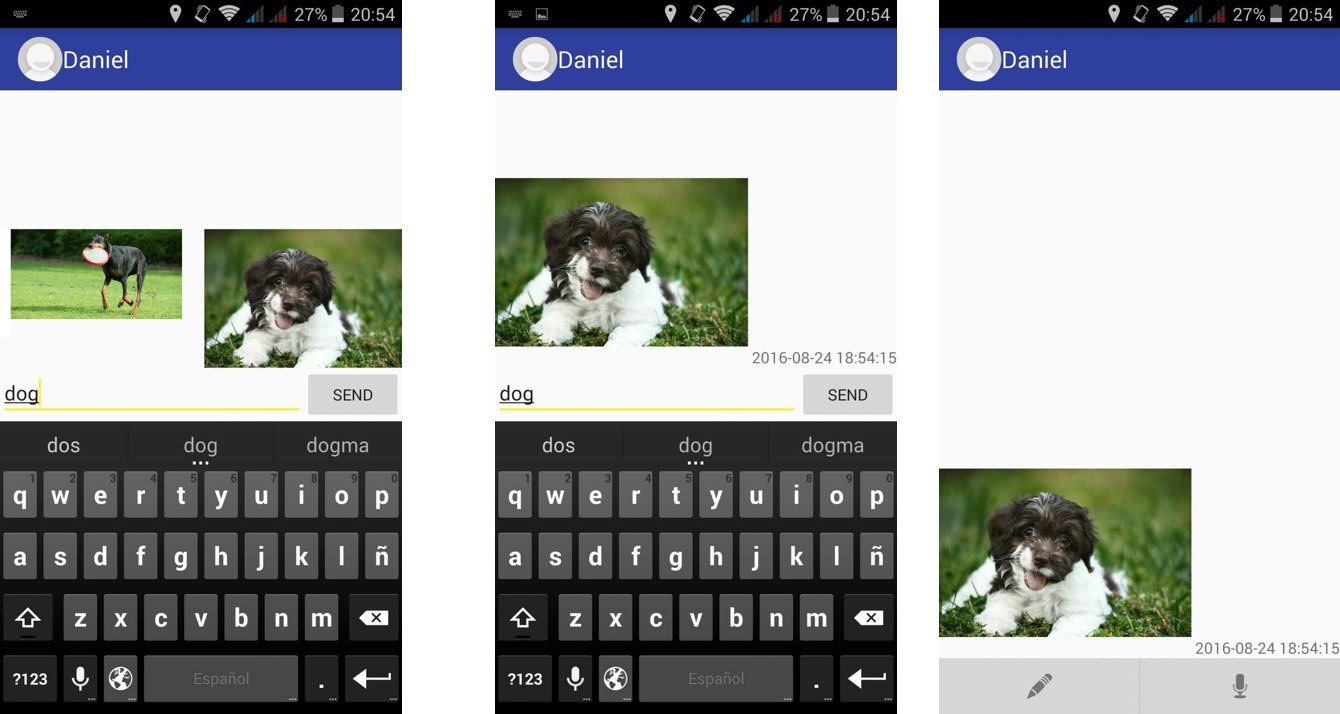
\includegraphics[width=0.9\textwidth]{./figures/interfaz-busqueda.jpg}
\caption{Interfaz búsqueda de imágenes}
\label{fig:interfaz-busqueda}
\end{center}
\end{figure}


\subsubsection{Tarea: Extraer información de las imágenes seleccionadas}

Para poder utilizar estas imágenes en el futuro dentro del sistema de recomendación, será necesario extraer información de las mismas. Para este propósito se utilizará Google Cloud Vision. Cloud Vision es una \ac{API} integrada en los servicios proporcionados por Google Cloud Platform la cual permite extraer entre otras cosas información relativa a imágenes tales como etiquetas junto con la probabilidad estimada por este sistema de que se adapten a la realidad. Proporcionan otras funcionalidades, pero en este caso la que resulta de utilidad es esta.

Se  muestra el proceso seguido para realizar la extracción de la información a una imagen mediante esta \ac{API} en el Listado \ref{code:ImageLabelDetectionTask}.\\

\lstinputlisting[texcl, caption = {Búsqueda de imágenes utilizando Custom Search}, language = Java, label = code:ImageLabelDetectionTask]{code/ImageLabelDetectionTask.java}

\subsubsection{Tarea: Integrar la búsqueda y el envío de imágenes}

Es necesario, que cuando se seleccione una imagen que procede de la web, se comprueba si ya existe esa imagen en el repositorio local para no volver a subirla y así no desperdiciar recursos. Además, cuando se seleccione una de estas imágenes será necesario enviarla utilizando los mecanismos desarrollados en la iteración anterior. En la Figura \ref{fig:ImageSelected} se muestra el flujo que se produce cuando un usuario selecciona una imagen, distinguiendo esencialmente dos casos. Por un lado encontramos el caso en el que la imagen existe actualmente en el repositorio, para lo cual se comprueba si o bien la imagen la ha proporcionado el sistema de recomendación, con lo cual ya tendría la clave del blob, o en caso contrario, se comprueba si el enlace completo de la imagen se encuentra en el servidor. Si no se cumple ninguna de las dos condiciones anteriores, entonces es necesario incluir la imagen en el servidor propio, y por tanto es necesario etiquetarla y subirla.

\begin{figure}[!h]
\begin{center}
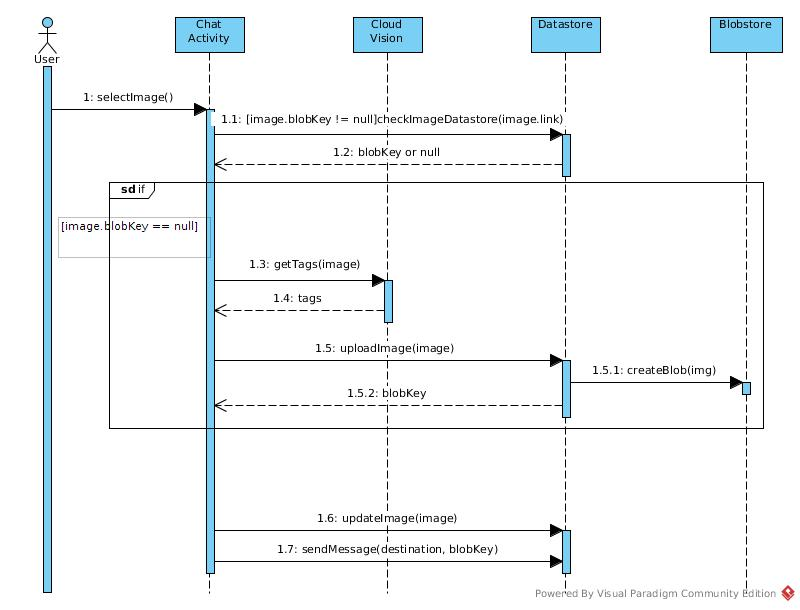
\includegraphics[width=1.1\textwidth]{./figures/ImageSelected.jpg}
\caption{Diagrama de secuencia selección de una imagen}
\label{fig:ImageSelected}
\end{center}
\end{figure}

 
\subsubsection{Tarea: Limpieza de la entrada}

En la Sección \ref{sec:sistema-recomendacion} ya se presentó la funcionalidad relativa al procesamiento de la entrada ya que es una parte muy importante para el sistema de recomendación, por lo que aquí simplemente se mostrará una pequeña descripción y el código encargado de realizar esta para no resultar repetitivos. Es necesario recordar que para esto se usará la \ac{BBDD} de Wordnet, que contiene información tanto de los significados de las palabras, como la relación entre estas  y sus sinónimos, e hiperónimos.

Este preprocesamiento esta destinado a eliminar las consideradas como \textit{stop words}, o palabras que no aportan semántica al lenguaje. Además, y con el propósito de estandarizar la entrada, se reducirán ciertas palabras a su raíz, como los verbos que se pasarán a forma infinitiva, o la eliminación de plurales. En el Listado \ref{code:cleanInput} se muestra el método \texttt{cleanInput} que es el encargado de limpiar la entrada.\\

\lstinputlisting[texcl, caption = {Limpieza de la entrada}, language = Java, label = code:cleanInput]{code/cleanInput.java}

\subsubsection{Tarea: Expansión de la entrada}

El proceso de expansión de la entrada tiene como objetivo el de extraer sinónimos de las diferentes palabras introducidas por los usuarios, así como las diferentes categorías en las que estas palabras se engloban (hiperónimos). En el Listado \ref{code:getSyns}, se muestra la obtención de los sinónimos, y en el Listado \ref{code:getHyper} se muestra la obtención de los hiperónimos.\\

\lstinputlisting[texcl, caption = {Obtención de los sinónimos}, language = Java, label = code:getSyns]{code/getSyns.java}

\lstinputlisting[texcl, caption = {Obtención de los hiperónimos}, language = Java, label = code:getHyper]{code/getHypers.java}

\subsubsection{Sprint Review}

Durante esta reunión se presentan los avances, presentando una aplicación que cumple con las características técnicas que se fijaron en un principio. Ya solo falta el último paso que es integrar el sistema de recomendación.

\subsubsection{Sprint Retrospective}

Se ha conseguido extraer una menor cantidad de información de la prevista inicialmente, por lo que se tendrá que replantear un poco el algoritmo de recomendación que en un principio se había planteado.

\subsection{Sprint 5}
A lo largo de este Sprint, se desarrollará la última y más importante pieza del proyecto, el Sistema de Recomendación. Tanto al principio del proyecto, como a lo largo del mismo, se ha ido dando forma a la idea de como debería funcionar el algoritmo, y los recursos y materiales utilizados, lo han sido debido a estas ideas (aunque se haya tenido que adaptar un poco). Pese a que la idea principal ya se tiene, ahora es necesario concretar y matizar estas en un algoritmo real, que utilizando los recursos a su disposición realice la mejor recomendación posible. El mecanismo que sigue el sistema desde la entrada por parte del usuario hasta la salida que el sistema le proporciona al mismo, ha sido explicado en la Sección \ref{sec:sistema-recomendacion}. Debido al carácter que tiene este módulo, se ha considerado necesario explicarlo por separado para que todo quede más claro. Además, en el Cuadro \ref{tab:user-story-7}. Además en la Figura \ref{fig:ImageSearch} se muestra un diagrama de secuencia en el que se puede observar el mecanismo final que se sigue cuando un usuario realiza una consulta.

\begin{table}[hp]
  \centering
  {\small
  \begin{tabular}{|p{0.4\textwidth} |p{0.4\textwidth} |}
\hline
\multicolumn{2}{|l|}{\cellcolor[HTML]{C0C0C0}{\textbf{Historia de usuario}}} \\ \hline
\textbf{Número:} 7          & \textbf{Rol: } Usuario        \\ \hline
\textbf{Esfuerzo:}           & \textbf{Iteración:} 5         \\ \hline
\multicolumn{2}{|p{0.8\textwidth}|}{\textbf{Nombre:} Imágenes adaptadas al perfil del usuario} \\ \hline
\multicolumn{2}{|p{0.8\textwidth}|}{\textbf{Desarrollador responsable:} Victor Gualdras de la Cruz} \\ \hline
\multicolumn{2}{|p{0.8\textwidth}|}{\textbf{Descripción:}\newline
Como usuario quiero que el sistema me proporcione las imágenes que mas se adapte a mis gustos y necesidades.
} \\ \hline
\multicolumn{2}{|p{0.8\textwidth}|}{\textbf{Validación:}\newline
Se realizan recomendaciones adaptadas a los usuarios y sus gustos.} \\ \hline
\multicolumn{2}{|p{0.8\textwidth}|}{\textbf{Tareas:}\newline
Tarea: Recomendar imágenes en base a la selección anterior del usuario.
Tarea: Relacionar usuarios con gustos en común y sugerir imágenes que otros usuarios relacionados hayan elegido.
Tarea: Analizar el contenido de la búsqueda y en base a este recomendar una serie de sitos donde buscar.
Tarea: Integrar todos los mecanismos anteriores en un único sistema de recomendación.
} \\ \hline
\end{tabular}
  }
  \caption{Historia de Usuario 7}
  \label{tab:user-story-7}
\end{table}

\begin{figure}[!h]
\begin{center}
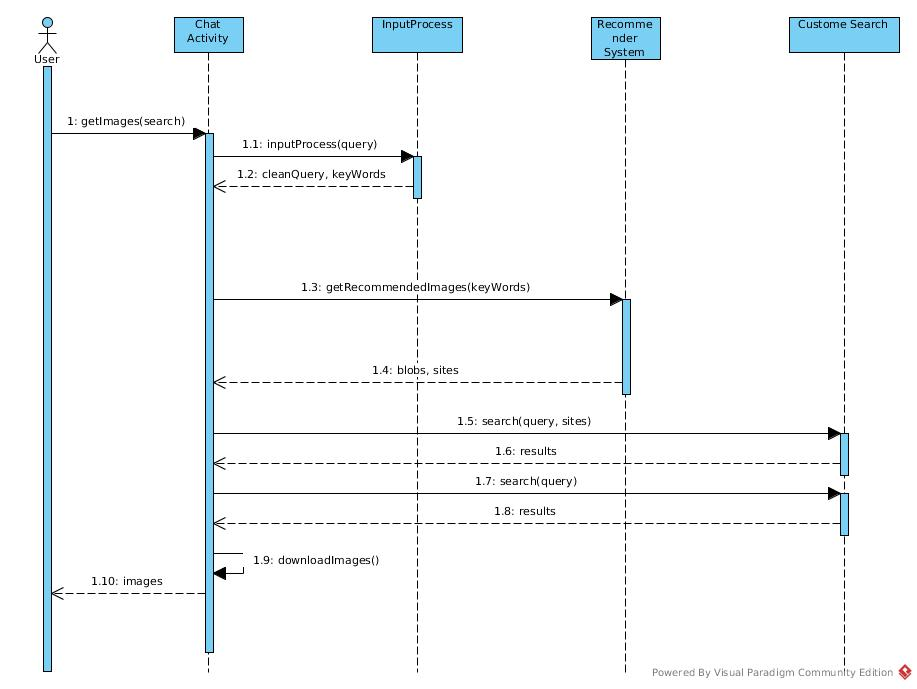
\includegraphics[width=1.1\textwidth]{./figures/ImageSearch.jpg}
\caption{Diagrama de secuencia de búsqueda del usuario}
\label{fig:ImageSearch}
\end{center}
\end{figure}

\subsubsection{Sprint Review}
Se ha entregado la versión finalizada del proyecto al Product Owner, el cual, ha falta de pruebas más intensivas para valorar el producto se ha mostrado bastante satisfecho con el resultado.


\subsubsection{Sprint Retrospective}
La mayor decepción para todos ha sido no haber podido realizar una cantidad de pruebas mayor, con los perfiles para los que estaba destinada la aplicación. Se espera sin embargo, poder subsanar este problema en el futuro.














